\documentclass[11pt,a4paper]{scrartcl} % Basisdokumentenklasse
\usepackage[ngerman]{babel}        % Deutsche Standardbezeichner und Trennung
\usepackage[latin1]{inputenc}      % Für Umlaute
\usepackage[T1]{fontenc}           % und ß
\usepackage{makeidx}               % Indexpaket
\usepackage{times}                 % Schönere Schriften, Achtung, nicht pslatex verwenden!
\usepackage{longtable}             % Lange Tabelle für Abkürzungsverzeichnis
\usepackage{graphics}              % EPS-Grafiken einbinden
\usepackage{theorem}               % Theorem-Optionen
\usepackage{bbding}
\usepackage{fancyvrb}              % Fancy-Verbatin für Programmlistings
\usepackage{booktabs}
%meine eigenen Pakete
\theoremstyle{break} % Zeilenumbruch nach Theorem
\newtheorem{mydef}{Definition}
%Fürs zeichenen
\usepackage{tikz}
\usetikzlibrary{shapes,arrows}
%Für schöne Algorithmen Darstellungen
\usepackage{listings}
%\usepackage{todonotes}
\usepackage{subfigure}
%- für multirow Tabellen
\usepackage{multirow}
%- für die schöne Darstellung von URLS
\usepackage{url}
%für schöne Formelumgebung
\usepackage{amssymb,amsmath}


\usepackage{boxedminipage}
%Um bei Code Unterschriften zu haben verwendeung von eigenem Listing Stilen (Kai)
%\input{content/listings}
%für mehrsoaltigen Text
\usepackage{multicol}
\usepackage{multirow}
%temp für eigenes comand
% hyperref ohne die Kästchen benutzen, sondern Links dunkelbalu zeigen
\usepackage{color}
\definecolor{lightgray}{gray}{0.9}
\definecolor{myg}{rgb}{213,201,216}
%Für linksiun Dokumenten
\usepackage[breaklinks=true,linkcolor=darkblue,menucolor=darkblue,urlcolor=darkblue]{hyperref}
%\usepackage{breakurl}

%YTe Box zur Interface Beschreibung 
\usepackage{float}
\floatstyle{boxed}
\newfloat{IDL}{thp}{loa}
\floatname{IDL}{Transformation Definition}

%20. 2. 12 Hurenkinder und Schusterjungen verhindern
\clubpenalty = 10000
\widowpenalty = 10000
\displaywidowpenalty = 10000


%%weitere Befhele innerhalb der IDL
\newcommand{\overview}[1]{\textbf{Overview: \\ }{#1}\\}
\newcommand{\arguments}[1]{\textbf{Supplied Arguments: \\ }{#1\\}}
\newcommand{\preCon}[1]{\textbf{Pre-Conditions:  \\}{#1\\}}
\newcommand{\postCon}[1]{\textbf{Results: \\ }{#1\\}}
\newcommand{\error}[1]{\textbf{Errors: \\}{#1\\}}
%eigene Comands für Begriffe:
\newcommand{\automais}{AutoMAIS}
%\newcommand{\staticDataSource}{static data source }
%\newcommand{\staticDataSources}{static data source }
%\newcommand{\dynamicDataSource}{dynamic data source }
%\newcommand{\dynamicDataSources}{dynamic data sources }

% data Connections für datenquellen
% data structuren für datenquellen
% inforamtion für datenquellen 
\newcommand{\information}{information}
\newcommand{\Information}{Information}
% measure
\newcommand{\measure}{measure }
\newcommand{\measures}{measures }
\newcommand{\Measure}{measure }
\newcommand{\Measures}{measures } 
% base measure 
\newcommand{\basemeasure}{base measure }
\newcommand{\basemeasures}{base measures }
\newcommand{\Basemeasure}{base measure }
\newcommand{\Basemeasures}{base measures }


 \newcommand\versicherung[1]{\chapter*{Versicherung}
\thispagestyle{empty}
Hiermit versichere ich, dass ich diese Arbeit selbst\"{a}ndig verfasst und keine anderen als die angegebenen Quellen und Hilfsmittel benutzt habe. Au{\ss}erdem versichere ich, dass ich die allgemeinen Prinzipien wissenschaftlicher Arbeit und Ver\"{o}ffentlichung, wie sie in den Leitlinien guter wissenschaftlicher Praxis der Carl von Ossietzky Universit\"{a}t Oldenburg festgelegt sind, befolgt habe.

\vspace{1.5cm}

#1, den 27. Februar 2012

\vspace*{-0.5cm}\hspace*{5.5cm}\hrulefill\\
\hspace*{6.5cm}\hfill Yvette Teiken \hfill\mbox{}
}


%\newcommand{\RZO}{R$_2$O}
% software engineering
\newcommand{\SE}{software engineering }
\newcommand{\se}{software engineering }

%\newcommand{\awNot}[1]{%
%\begin{boxedminipage}[t]{14cm}
%#1
%\end{boxedminipage}
%   
%}




%Komondo um den Index Eintrag fett zu machen. Benutzt man bei der Definition des Begriffs kommt von RST
\newcommand{\defkey}[1]{\textbf{#1}\index{#1|textbf}}

\title{Dokumentation von BI Projekten} 
%\title{ AutoMais  \\ Automatische Modellgetriebene Analytische Informationssysteme} % Titel der Dissertation
\author{Dr. Yvette Teiken}

                % Tag der Disputation

\makeindex



%Befehl um nur bestimmte Kapitel zu inkludieren um sie zu AW zu geben
%\includeonly{content/evaluation,content/Summary}

% Das eigentliche Dokument
\begin{document}

% Anfang des Dokuments
\maketitle              % Offizielle Titelseite der Uni, bei Abgabe auskommentieren!
%eine leere seite einfügen ohne Seitennummer
%\thispagestyle{empty}
%\cleardoublepage
%\pagenumbering{Roman}   % Römische Seitenzahlen für den Anfang
%\setcounter{page}{5}    % Bei römisch V anfangen	


% Zusammenfassung und Abstract

%\input{content/Dank.tex}
%\input{content/abstract.tex}



% Inhaltsverzeichnis

%\tableofcontents

\cleardoublepage        % Danach auf ungerader Seite weitermachen
\pagenumbering{arabic}  % Arabische Seitenzahlen starten neu

\section{Einleitung}
Dieses Dokument beschreibt wie BI Projekte durchgef�hrt werden sollen. Dieses Dokument stellt Grundlagen f�r die Dokumentation bereit. Hier werden Checklisten und Best Practices gesammelt und zusammengef�gt.


\chapter{Allgemeine Architektur}
In diesem Kapitel wird die generelle Architektur der L�sung bzw. des Projekts beschrieben.
\section{Datenanlieferung}
Was ist das besondere an der Anlieferung, wo und wie muss das ber�cksichtigt werden
%\begin{itemize}
%\item[\Square] offener Punkt
%\item[\XBox] angekreuzter Punkt
%\item[\CheckedBox] abgehakter Punkt
%\end{itemize}
\begin{itemize}
	\itemtodo Wie werden die Daten angeliefert?
	\itemtodo Werden alle Daten gleich angeliefert bzw. welche Ausnahmen gibt es?
	\itemtodo Gibt es besondere Anforderungen an Sicherheit bzw. Aufbewahrungspflichten?
	\itemdone Das ist schon erledigt.
\end{itemize}

\section{Abgeleitete Architektur}
Wie sieht die Architektur aus? Welche Schichten gibt es? Wie ist der Datenfluss zwischen den Schichten? Wie ist der Bezug zu unseren Best Practices?

\section{Logging und Bereinigung}
\begin{itemize}
	\itemtodo Wie soll das Logging laufen?
	\itemtodo Was sind die Prozesse?
	\itemtodo Welche Tabellen werden beteiligt?
\end{itemize}


\section{Zentrale Datenhaltung}
\begin{itemize}
	\itemtodo Wie ist das zentrale Analyseformat (Star, Data Vault oder was anderes?)
	\itemtodo Wie wird mit Business Keys umgegangen?
	\itemtodo Wie werden Stammdaten abgeleitet?
\end{itemize}

\section{Berichte}
Welche Berichte gibt es? WIe werden diese erzeugt?


\chapter{Architektur- und Programmierrichtlinien}
In diesem Abschnitt werden Richtlinien und Best Practices gesammelt.

\section{Technichnical IDs}
F�r die Vergabe von technischen Schl�sseln gibt es zwei Alternativen als numeric oder als Guid

Eigenschaften von GUIDs
\begin{itemize}
	\item Sind global eindeutig im System, ein Item ist immer eindeutig identifizierbar
	\item neue Guids im SSIS kann man mittels abgeleiteter Spalte hinzuf�gen zum Datenfluss
	\item Sind in der Geschwindigkeit bei der Verarbeitung gef�hlt langsamer
	\item Bei der DAK und im Data Vault Kontext werden Guids f�r technische IDs verwendet. 
\end{itemize}

Eigenschaften von numerischen technischen Schl�sseln
\begin{itemize}
	\item K�nnen automatisch erzeugt werden beim Einf�gen in der Tabelle
	\item Sind nur eindeutig pro Tabelle und nicht im System
	\item Sind in der Verarbeitung etwas angenehmer
\end{itemize}


\section{Stagging in Tabellen}

\section{Formatierungen}
Es gibt zwei Alternativen hierf�r:

	\subsection{Mittels SSIS:} Die Konvertierungen werden mittels SISS Komponenten durchgef�hrt.Wie dies geht, hier \ref{DustinRyan} vorgestellt. Hier verwendet man abgeleitete Spalten f�r
	
	\begin{lstlisting}[language=SQL,label=listFormatSISS, caption=Formatierung mit SISS und Behandlung von leeren Werten]
% reine Pr�fung
(DT_UI4)Alter == (DT_UI4)Alter ? 1 : 0
% hier wird es automatisch auf den konvertireten Wert gelegt
(DT_UI4)Alter == (DT_UI4)Alter ? (DT_UI4)Alter : 0
\end{lstlisting}
	\textbf{Mittels SQL:} Die Daten werden als Text in eine DB integriert und dann danach mittels SQL Konvertierungen in das Zielformat �berf�hrt. 




\subsection{Extraktion von Daten} \label{BP_Extract}


\subsection{Daten bereinigen mittels Data Profiling Task}
Um den Task verwenden zu k�nnen, m�ssen die Daten in einer ADO.NET Datenquelle vorhanden sein. Es hilft auch nur um die Daten einsch�tzen zu k�nnen. Die Ergebnisse liegen dann in einer XML Datei und k�nnen betrachtet werden. Man sieht in den Ergebnisse eine Verteilung von Werten.

\subsubsection{Daten bereinigen mittels DQS}
Der Ansatz an sich ist ganz cool. Mann kann Dom�nen festlegen und Wertebereiche und Regeln zu den Werten festlegen. Der Client an sich ist relativ langsam und etwas fehleranf�llig und absturzgef�hrdet. Ein kontinuierliches Arbeiten mit dem Client ist fast unm�glich.\\
 
In der Abbildung \ref{fig:KnowledgeGender} werden die m�glichen Auspr�gungen beschrieben. Es k�nnen Synonyme verwendet werden, diese werden dann auf den Repr�sentanten abgebildet. Auch k�nnen Regeln festgelegt werden. Wie im Beispiel Alter zu sehen ist. Hier wird der Wertebereich entsprechen eingeschr�nkt.

\begin{figure}[htbp]
	\centering
		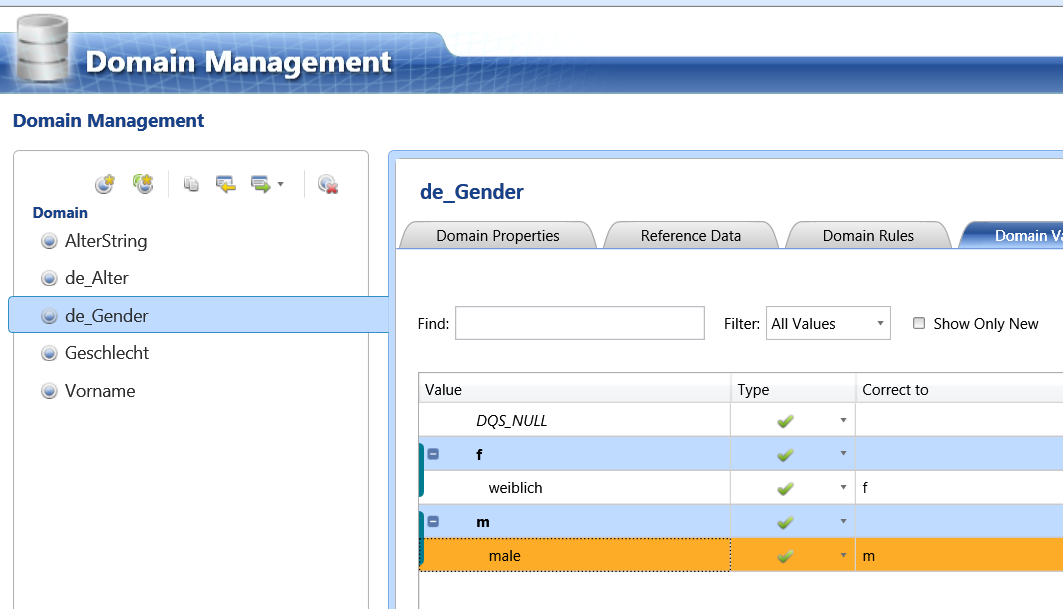
\includegraphics[width=0.80\textwidth]{doku/Bilder/KnowledgeGender.PNG}
	\caption{Dom�n Geschlecht mit Werten}
	\label{fig:KnowledgeGender}
\end{figure}

Die Bereinigung der Daten kann dann im SISS vorgenommen werden, wie es in Abbildung \ref{fig:SISS_DQS_Task} gezeigt ist. Der Task an sich ist recht sch�n. Man kann die Dom�ne zu einer Spalte angeben  und alle Regelen, die in der Kowledgebase verf�gbar sind werden angewendet. Als Ergebnis erh�lt man dann korrigierte oder aussortierte Daten, wie in Abbildung \ref{fig:DQS_Result} zu sehen ist.\footnote{In meinem Beispiel hat die Abbildung von Geschlecht m�nnlich nicht funktioniert und es wurde die ID der Spalte verwendet. Ich konnte nicht nachvollziehen warum das so ist.}

\begin{figure}
	\centering
		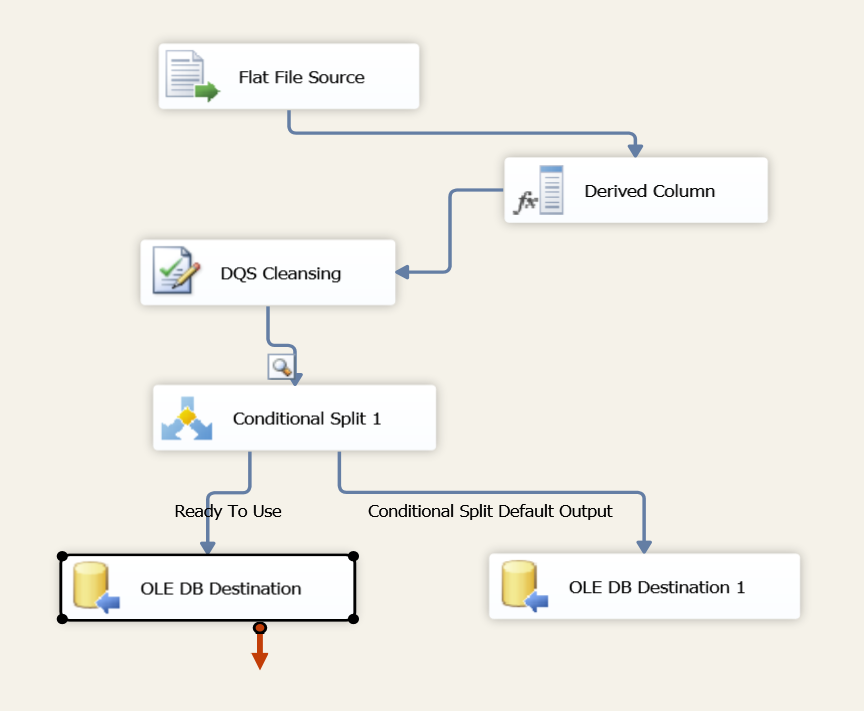
\includegraphics[width=1.00\textwidth]{doku/Bilder/SISS_DQS_Task.PNG}
	\caption{DQS Task in SISS}
	\label{fig:SISS_DQS_Task}
\end{figure}

\begin{figure}
	\centering
		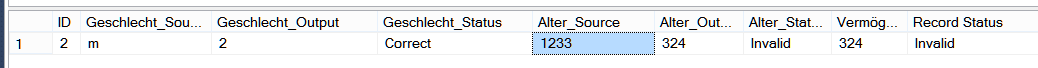
\includegraphics[width=1.00\textwidth]{doku/Bilder/DQS_Result.PNG}
	\caption{DQS Ergebins, invalide Daten}
	\label{fig:DQS_Result}
\end{figure}

%\include{content/Introduction}
% Der eigentliche Inhalt
%Grundlagen
%\include{content/Grundlagen}
%Fallstudie  
%\include{content/ExampleAisCreation}
%\include{content/relatedWork}
%der Ansatz an sich 
%\include{content/autoMAIS}


%\include{content/processModel}

%%achuting hier große Überschrift
%-- Kennzahlen
%\include{content/measures}
% -- Analyse Schema 
%\include{content/AnalyseSchema}
% -- Hierarchien

%\include{content/Hierarchien}

%-- Datenquellen
%\include{content/Datenquellen}


%--Datenquellen Transformationen

%\include{content/DataTransformation}

%--Datenqualität
%\include{content/DatenQualitaet}
%Integrationskapitel
%\include{content/Integration}
%\include{content/architecture}
%\include{content/Transformation}
%\include{content/ConclusionConcept}
%Evaluation
%\include{content/evaluation}
%\include{content/Summary}

%\include{content/Appendix}

% Verzeichnisse am Ende, erst das Glossar
%\include{content/glossar}






% Dann die Abkürzungen
%\include{content/abkuerzungen}

% Weiter mit Abbildungen
%\cleardoublepage
%\addcontentsline{toc}{chapter}{Figures} % Sowohl im Inhaltsverzeichnis als auch als
%\renewcommand{\listfigurename}{Figures} % Überschrift als "Abbildungen" ohne -verzeichnis
%\listoffigures

% Schließlich Literatur
%\cleardoublepage
%\nocite{*}
%\addcontentsline{toc}{chapter}{References} % Soll als "Literatur" auftauchen
%\bibliographystyle{alphadin}                 % Unser Standard-Bibliopgraphiestyle
%24.4. Versuch wegen englischer literatur
%\bibliographystyle{alpha}  
%\renewcommand{\bibname}{References}        % Auch als Überschrift soll "Literatur" erscheinen
%\bibliography{content/bibliographie}            % Literaturverzeichnis einbinden

% Und ganz am Ende der Index
%\cleardoublepage
%\addcontentsline{toc}{chapter}{Index} % Der auch Index heißen soll
%\printindex
%\input{content/index.tex}                     % Index einbinden, vorher aber mit makeindex erzeugen!
%so geht index mit dem Texniccenter "%bm.idx" -o %tm.ind -t %tm.ilg 

%bm.idx" -s olwir.ist -o %tm.ind -t %tm.ilg 


%\versicherung{Oldenburg}
\end{document}

